
\documentclass[12pt]{article}
\usepackage{geometry} % see geometry.pdf on how to lay out the page. There's lots.
\geometry{a4paper} % or letter or a5paper or ... etc
\usepackage{amsmath}
\usepackage{braket}
\usepackage{graphicx}
\usepackage{color}


\begin{document}
\setlength{\parindent}{0 pt}

\begin{center}
\textbf{$S_{11}$ derivation for lumped element parallel LCR circuit}
\end{center}

From Pozar: \\
Signal on a transmission line looking into an impedance $Z_l$

\[
V(z) = V_0^+e^{i\beta z} + V_0^-e^{-i \beta z}
\]

\[
I(z) = I_0^+ e^{i\beta z} - I_0^- e^{- i \beta z} = \frac{V_0^+}{Z_0}e^{i\beta z} - \frac{V_0^-}{Z_0}e^{-i \beta z}
\]

\begin{figure}[htbp]
\begin{center}
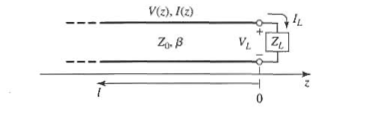
\includegraphics[scale = .75]{TxLinePozar}
\caption{default}
\label{default}
\end{center}
\end{figure}

\[
V(0) = I(0) Z_l \rightarrow Z_l = \frac{V(0)}{I(0)} = \frac{V_0^+ + V_0^-}{V_0^+ - V_0^-}Z_0
\]

Solve for $V_0^-$


\[
V_0^- = \frac{Z_l - Z_0}{Z_l + Z_0}V_0^+
\]

\[
S_{11} = \frac{V_0^-}{V_0^+} = \frac{Z_l - Z_0}{Z_l + Z_0}
\]

Calculate the impedance of the parallel LCR resonator

\[
Z_r = \left[\frac{1}{Z_L} + \frac{1}{Z_c} + \frac{1}{R}\right]^{-1}
\]

\[
Z_r = \left[-\frac{i}{\omega L} + i \omega C + \frac{1}{R} \right]^{-1}
\]

\[
Z_r = \left[-\frac{i}{\omega L} + \frac{i \omega^2 LC}{\omega L} + \frac{1}{R}\right]^{-1}
\]

\[
Z_r = \left[\frac{i R (\omega^2 LC - 1) + \omega L}{R\omega L}\right]^{-1}
\]

Equatiing $(LC)^{-1} = \omega_0^2$ and inverting...

\[
Z_r = \frac{R\omega L}{\omega L + i R(\omega^2/\omega_0^2 - 1)}
\]

\[
Z_r = \frac{R}{1 + i \frac{R}{\omega L}(\omega^2/\omega_0^2 - 1)}
\]

Rewrite using the Q of the resonator

\[
Q_r = \omega_0 R C = R \sqrt{\frac{C}{L}} = \frac{R}{\omega_0 L}
\]

\[
Z_r = \frac{R}{1 + i \frac{R}{\omega_0 L}(\omega/\omega_0 - \omega_0/\omega)}
\]

\[
Z_r = \frac{R}{1 + iQ_r(\frac{\omega^2 - \omega_0^2}{\omega \omega_0})}
\]

Take $\omega \approx \omega_0$

\[
Z_r = \frac{R}{1 + iQ_r(\frac{(\omega + \omega_0)(\omega - \omega_0)}{\omega \omega_0})} = \frac{R}{1 + i2 Q_r(\frac{\omega - \omega_0}{\omega_0})}
\]

\[
x = \frac{\omega - \omega_0}{\omega_0}
\]

\[
Z_r = \frac{R}{1 +i 2 Q_r x}
\]

\[
Z_r = \frac{R}{1 + 4 Q_r^2 x^2} - i \frac{ 2 R Q_r x}{1 + 4 Q_r^2 x^2}
\]

Looking at the Norton Equivalent

\[
R_t = \frac{1+ \omega^2 C_c^2 R_l^2}{\omega^2 C_c^2 R_l} \approx \frac{1}{\omega^2 C_c^2 R_l}
\]

\[
C_t  = \frac{ C_c}{1 + \omega^2 C_c^2 R_l^2} \approx C_c
\]

\[
Q_c = \omega R_t C_r = \frac{Q_r R_t}{R}
\]

\[
\frac{Q_r}{Q_c} = \frac{R}{R_t}
\]

The impedance has been transformed by the input capacitor from $Z_0 \rightarrow R_t$. So $S_{11}$ now equals

\[
S_{11} = \frac{Z_r - R_t}{Z_r + R_t} = \frac{ Z_r/R_t - 1}{Z_r/R_t + 1}
\]

\[
Z_r/R_t = \frac{R/R_t}{1 + 2iQ_r x} = \frac{Q_r/Q_c}{1 + 2i Q_r x}
\]

\[
S_{11} = \frac{\frac{Q_r/Q_c}{1 + 2i Q_r x} - 1}{\frac{Q_r/Q_c}{1 + 2i Q_r x} + 1}
\]

factor out $1/(Q_c + 2I Q_c Q_r x)$

\[
S_{11} = \frac{ Q_r - (Q_c + 2i Q_r Q_c x)}{Q_r + (Q_c + 2i Q_r Q_c x)}
\] 

\[
S_{11} = \frac{ Q_r - Q_c - 2i Q_r Q_c x}{Q_r + Q_c + 2i Q_r Q_c x}
\]


\[
S_{11} = \frac{Q_r - Q_c}{Q_r + Q_c} \left(\frac{1 - 2i \frac{Q_r Q_c}{Q_r - Q_c} x}{1 + 2i \frac{Q_r Q_c}{Q_r + Q_c}x}\right)
\]

\[
S_{11} = S_{11}^{min} \frac{1 - 2i Q_{eff} x}{1 + 2i Q_{t} x}
\]

\[
S_{11}^{min} =  \frac{Q_r - Q_c}{Q_r + Q_c} 
\]

\[
Q_{eff} = \frac{Q_r Q_c}{Q_r - Q_c}
\]

\[
Q_t = \frac{Q_r Q_c}{Q_r + Q_c}
\]
\end{document}